\subsection{Theory of spectral clustering}\label{sec:spectral_theory}

Spectral clustering begins with embedding all data in a new space using the eigenvectors.
In this new space the clustering a standard clustering will be performed.
Embedding is the result of relaxing the criteria that would precisely
to identify infinitely separated groups to estimate the members  groups that may have some connection.
This is best described in \cite{luxburg2007spectraltutorial}, a short summary is given here.

Let us imagine a graph, disconnected in \(n\) clusters.
The initial aim is to identify which of the disconnected components each point belongs to.
The objective used for a good clustering will be the NCut objective;
\begin{equation}
    \text{NCut} = \sum_k\frac{W(A_k, \bar{A_k})}{|A_k|}
\end{equation}
Where \(W(A_k, \bar{A_k})\) measures the strength of the connections that must be
broken in order to separate the cluster \(A_k\) from the graph
and \(|A_k|\) corresponds to the number of elements in \(A_k\).

Membership of cluster \(A_k\) will be determined by the indicator vector \(h_k\);
\begin{equation}
    h_{i, k}= 
    \begin{cases}
        1/\sqrt{|A_k|},& \text{if point } i \in A_k \\
        0,              & \text{otherwise}
    \end{cases}
\end{equation}
where \(|A_k|\) is the number of points in set \(A_k\).
A pair of points is assigned an affinity, \(a_{i,j} = a_{j, i}\),
of either \(1\) for connected \(i\) and \(j\) or \(0\) 
if points \(i\) and \(j\) are unconnected.

The graph is represented by the graph Laplacian, a square
matrix with as many rows and columns as there are points.
On \(i\)th diagonal it holds the value \(\sum_j a_{i, j}\),
which is the degree of the vertex \(i\).
Off the diagonal it has the negative affinity; \(-a_{i, j}\).
\begin{equation}\label{eqn:laplacian}
    L = 
    \begin{pmatrix}
        z_0 & -a_{0,1} & -a_{0,2} & \hdots \\
        -a_{0,1} & z_1 & -a_{1,2} & \\
        -a_{0,2} & -a_{1,2} & z_2 & \\
        \vdots   &          &     & \ddots 
    \end{pmatrix}
\end{equation}

Notice that this is a real symmetric matrix,
and therefore all its eigenvalues are real.

Considering just one cluster we find that when the Laplacian is multiplied by two indicator vectors
the result is the function that NCut seeks to minimise for that cluster.
\begin{equation}
    h_k'Lh_k = \frac{1}{|A_k|}\sum_{i \in A_k, j \in A_k} \left(\delta_{i, j}\sum_{l} a_{l, i} - a_{i, j} \right) = \frac{W(A_k, \bar{A_k})}{|A_k|}
\end{equation}
Stack the indicator vectors into a matrix;
\begin{equation} h'_k L h_k = (H'L H)_{kk}\end{equation}
and the NCut aim described earlier becomes the trace;
\begin{equation} \text{NCut}(A_1,A_2, \dots A_n) \equiv \frac{1}{2} \sum_{i=1}^n \frac{W(A_i, \bar{A_i})}{|A_i|} = \text{Tr}(H'LH)\end{equation}
Where \(H'H = I\).
Trace minimisation in this form is done
by finding the eigenvectors of \(L\) with smallest 
eigenvalues.

Generalising this to a graph that is not disconnected
only requires relaxing the requirements on the form of the indicator vectors; \(h_k\).

Once these indicator vectors have been created the position of the points in the embedding space is determined.
Each indicator vector has as many elements as there are points to be clustered,
so the coordinates of a point are the corresponding elements or the indicator vectors.
Using the positions in embedding space the points can be gathered agglomeratively,
this part is not a relaxation of a well defined objective.
\subsubsection{Impact of \(p_T\) factors}
In the case of reconstructed particles, a possible input to the affinity measure is the \(p_T\) of the particles.
A format commonly used for the distance is;
\begin{equation}d_{i,j} = \text{min}(p_{T,i}^{2x}, p_{T,j}^{2x}) \distancedeltar{}_{i,j}\end{equation}
where \(\distancedeltar{}_{i,j}\) is an angular distance.
This is discussed from a practical standpoint in section~\ref{sec:spectralmethodalgo},
from a theoretical standpoint it is important to investigate the impact of the \(p_T\) factor on the eigenvalue equations.
There are a number of different ways of converting a distance measure into an affinity,
for now only one will be considered \(a_{i,j} = 1/d_{i,j}\).

Starting with the Laplacian a relation between the size of the eigenvalues and the affinities in each group can be uncovered.
% The Laplacian has the form \(L = D -A\), as we are already using \(d\) to mean distance,
Let us take \(z_i = \sum_{j\neq i} a_{i,j}\) where it is understood that by default any sum goes over all node (i.e. particle) indices.
From this point onward it is also assumed that all \(a_{i,i} = 0\), so such sums can omit the \(i \ne j\).
With this, equation~\ref{eqn:laplacian} can be rewritten as
\begin{equation}
    L = 
    \begin{pmatrix}
        z_0 & -a_{0,1} & -a_{0,2} & \hdots \\
        -a_{0,1} & z_1 & -a_{1,2} & \\
        -a_{0,2} & -a_{1,2} & z_2 & \\
        \vdots   &          &     & \ddots 
    \end{pmatrix}
\end{equation}

Now imagine a group that includes the first \(q\) nodes,
its relaxed indicator vector approximately contains two values; \(-Q_0\) for nodes \(0\) to \(q\) inclusive
and \(Q_1\) for nodes \(q+1\) to \(n\) inclusive,  where \(Q_{0/1} > 0\).
As the ordering of the nodes is arbitrary (the rows and columns can have any order)
conclusions drawn for this hold for any group containing \(q\) nodes.
This must be approximate because we do not require that the \(q\) nodes are perfectly separated (the model is relaxed),
there for the eigenvalue equation is a relaxation.

The eigenvalue equation has the form
\begin{equation}
    \begin{pmatrix}
        z_0 & -a_{0,1} & -a_{0,2} & \hdots \\
        -a_{0,1} & z_1 & -a_{1,2} & \\
        -a_{0,2} & -a_{1,2} & z_2 & \\
        \vdots   &          &     & \ddots 
    \end{pmatrix}
    \begin{pmatrix}
        -Q_0 \\
        -Q_0 \\
        \vdots \\
        Q_1 \\
    \end{pmatrix}
    \approx \lambda
    \begin{pmatrix}
        -Q_0 \\
        -Q_0 \\
        \vdots \\
        Q_1 \\
    \end{pmatrix}
\end{equation}.

The simultaneous equations that come from this can be simplified into two forms.
The first \(q\), where \(i \leq q\), take the form
\begin{equation}-Q_0 \lambda \approx Q_0 \sum_{j \leq q} a_{i,j} - Q_0 z_i - Q_1\sum_{j>q} a_{i,j}\end{equation}
\begin{equation}\lambda \approx \left(1 + \frac{Q_1}{Q_0}\right)\sum_{j>q} a_{i,j}\end{equation}.
In a similar manner the remaining simultaneous equations, where \(k > q\) have the form
\begin{equation}\lambda \approx \left(1 + \frac{Q_0}{Q_1}\right)\sum_{j\leq q} a_{k,j}\end{equation}.
In both cases the sum is over affinities that attach to the node associated with the row
and cross the cluster boundary.

Clearly the size of the eigenvalue will be related to the size of the affinities that cross the boundary.
More subtly, if the number of elements in each group differs strongly then the values of \(Q_0\) and \(Q_1\)
will need to differ more to compensate.
Approximating all the affinities to the same value
\begin{equation}\left(1 + \frac{Q_1}{Q_0}\right)qa = \left(1 + \frac{Q_0}{Q_1}\right)(n-q)a\end{equation}
\begin{equation}\left(1 + \frac{Q_1}{Q_0}\right) = \left(1 + \left(\frac{Q_1}{Q_0}\right)^{-1}\right)\frac{q-n}{q}\end{equation}
it can be seen that as \(\frac{q-n}{q}\) deviates from \(1\) the solution grows the left side faster than it shrinks the right.
This will also tend to increase the value of \(\lambda\).

So essentially a split associated with a small eigenvalue will minimise the value of the crossing affinities
and create groups with equal number of members.
Returning to the idea of the influence of \(p_T\), this will have impact on the former condition but not the latter.
Taking \(a_{i,j} \sim 1/\text{min}(p_{T,i}^{2x}, p_{T,j}^{2x})\) with \(x>0\) affinities involving a low \(p_T\)
particle will be larger, so the placement of soft emissions will be important.
Alternatively, with \(x < 0\) affinities involving one high \(p_T\) particle will be larger,
so the placement of hard emissions will be most important.

This has found the role of \(p_T\) in an unnormalised laplacian,
the same steps can be taken for the \textbf{symmetric laplacian}; \(L = D^{-1/2}(D -A) D^{-1/2}\).
\begin{equation}
    L_\text{symm} = 
    \begin{pmatrix}
        1 & -a_{0,1}(z_0z_1)^{-1/2} & -a_{0,2}(z_0z_2)^{-1/2} & \hdots \\
        -a_{0,1}(z_0z_1)^{-1/2} & 1 & -a_{1,2}(z_1z_2)^{-1/2} & \\
        -a_{0,2}(z_0z_2)^{-1/2} & -a_{1,2}(z_1z_2)^{-1/2} & 1 & \\
        \vdots   &          &     & \ddots 
    \end{pmatrix}
\end{equation}

Considering the same group of the first \(q\) rows the forms of the simultaneous equations are;
for \(i \leq q\)
\begin{equation}\label{eqn:symm_lamb1}
\lambda \approx 1 + z_i^{-1/2} \left(\frac{Q_1}{Q_0}\sum_{j>q}a_{i,j}z_j^{-1/2} - \sum_{j \leq q} a_{i,j}z_j^{-1/2}\right).
\end{equation}
Notice that the first sum is over affinities that cross out of the group, divided by the root of the connectedness of the outside node,
(\(z_j\) can be seen as the connectedness of node \(j\)), the second sum is over affinities contained within the first \(q\) nodes,
also divided by the root of their connectedness.

Then for \(k > q\)
\begin{equation} \lambda \approx 1 + z_k^{-1/2} \left(\frac{Q_0}{Q_1}\sum_{j\leq q}a_{k,j}z_j^{-1/2} - \sum_{j > q} a_{k,j}z_j^{-1/2}\right).\end{equation}
Again the first sum is over affinities that cross the group, and now the second sum is over affinities not in the first \(q\) nodes.
Now finding the impact of \(p_T\) looks rather more complicated,
so it will be addressed in stages.
Firstly consider \(z_j = \sum_i a_{i,j} \sim \sum_i 1/\text{min}(p_{Ti}^{2x}, p_{Tj}^{2x}) \),
it's behaviour splits into 4 categories.
Consider \(N_j(p_T)\) to be roughly the \(p_T\) of a node that node \(j\) is connected to (Neighbour).
Also, let nodes on average have the equivalent of \(c\) connections, where \(0 \leq c \leq n\).
\begin{center}  % is x positive v.s. negative??
    \begin{tabular}{c | c c}
                & \(p_{Tj} < N_j(p_T)\) & \(p_{Tj} > N_j(p_T)\) \\
        \hline
        \(x>0\) & \(z_j \sim cp_{Tj}^{-2x}\) therefore \(z_j^{-1/2} \sim c^{-1/2} p_{Tj}^{x}\) & \(z_j \sim cN_j(p_T)^{-2x}\) therefore \(z_j^{-1/2} \sim c^{-1/2}N_j(p_T)^{x}\)\\
        \(x<0\) & \(z_j \sim cN_j(p_T)^{-2x}\) therefore \(z_j^{-1/2} \sim c^{-1/2}N_j(p_T)^{x}\) & \(z_j \sim cp_{Tj}^{-2x}\) therefore \(z_j^{-1/2} \sim c^{-1/2} p_{Tj}^{x}\)\\
    \end{tabular}
\end{center}
The first sum in equation~\ref{eqn:symm_lamb1} is \(\sum_{j>q}a_{i,j} z_j^{-1/2}\),
where \(i\) is in the first \(q\) nodes and \(j\) is always outside the first \(q\) nodes.
Let \(w_{i} = \sum_{j>q}a_{i,j} z_j^{-1/2}\).
If connections were randomly allocated after clustering then the probability of a connection crossing between clusters would be \(q(n-q)/n(n-q)\).
However as clustering is supposed to avoid breaking connections the probability number of crossing connections will be lower than this.
Call this \(\chi\), so that the sum \(\sum_{j>q}a_{i,j}\) has on average \(\chi c\) non zero terms.
A similar table is constructed for \(w_{i}\);
\begin{center}
    \begin{tabular}{c | c c}
                & For most \(j\); \(p_{Tj} < p_{Ti}\) & For most \(j\); \(p_{Tj} > p_{Ti}\) \\
        \hline
        \(x>0\) & \(w_{i} \sim \chi c^{1/2}p_{Tj}^{-x}\) & \(w_{i} \sim \chi c^{1/2}N_j(p_T)^x p_{Ti}^{-2x}\)\\
        \(x<0\) & \(w_{i} \sim \chi c^{1/2}N_j(p_T)^x p_{Ti}^{-2x}\)& \(w_{i} \sim \chi c^{1/2}p_{Tj}^{-x}\)
    \end{tabular}
\end{center}

Note that from the perspective of node \(i\) connected to node \(j\)
\(N_j(p_T)\) relates to the \(p_T\) two steps away in the direction of \(j\).

The other sums in equation~\ref{eqn:symm_lamb1} have similar form,
the distinction being is indices \(i\) and \(j\) belong to the same or opposing clusters.
This changes the prefactor, \(\chi\), as it is no longer a sum over crossing vertices, 
but otherwise the algebra will be the same as there are no assumptions about group membership in it.

The table is recast for those two cases, and the entries are described in terms of the influence of \(p_T\)
values on the magnitude of the sum.
Firstly, when both indices belong to the same cluster the sum is subtracted from the value of the eigenvalue. As such larger sums are favoured.
\begin{center}
    \begin{tabular}{c | p{0.45\textwidth} p{0.45\textwidth}}
                & Node \(i\) is high \(p_T\) so mostly \(p_{Tj} < p_{Ti}\) & Node \(i\) is low \(p_T\) so mostly \(p_{Tj} > p_{Ti}\) \\
        \hline
        \(x>0\) & The smaller the \(p_T\) of a node connected to \(i\) the greater its contribution to the sum. The clustering is favoured when \(i\) connects to many soft nodes. The harder \(p_{Ti}\) is not used directly.&
        The larger the neighbourhood \(p_T\) for a node connected to \(i\) in comparison to soft \(p_{Ti}\) the greater its contribution to the sum. The clustering is favoured when nodes connecting to \(i\) sit in a higher \(p_T\) neighbourhood. The harder \(p_{Tj}\) is not used directly.\\
        \(x < 0\) &  The larger the neighbourhood \(p_T\) for a node connected to \(i\) in comparison to hard \(p_{Ti}\) the greater its contribution to the sum. The clustering is favoured when nodes connecting to \(i\) sit in a higher \(p_T\) neighbourhood. The softer \(p_{Tj}\) is not used directly. &
        The smaller the \(p_T\) of a node connected to \(i\) the greater its contribution to the sum. The clustering is favoured when \(i\) connects to many soft nodes. The softer \(p_{Ti}\) is not used directly.\\
    \end{tabular}
\end{center}

The difference between \(x > 0\) and \(x < 0\) can be summarised as \(x > 0\) indicates that things
of differing scales should be connected and the highest \(p_T\)s should not reduce any connectedness.
On the other hand \(x < 0\) indicates that things of the same scale should be clustered together and the lowest \(p_T\)s should not reduce connectedness.


The sums that cross between groups are added to the value of the eigenvalue,
so increasing the value of the sum disfavours the clustering.
This symmetry means that the implications for \(x > 0\) or \(x < 0\) will be the same as summarised above.

%\subsubsection{Distances in Physical space}\label{sec:distance_in_physical}
%In order to test the best way to measure distance between two particles
%there are two simple metrics
%that should grow in an ordinal manner with distance.
%
%The first would be the ROC-AUC (Receiver Operating Characteristic - Area Under Curve),
%for the distance measure between two particles predicting the particles being descendent from the same
%\bthing{quark}.
%A ROC-AUC is a number between \(0\) and \(1\) measures how well a predictor matches the truth labels~\cite{Fawcett06anintroduction}.
%This can be thought of as a measure of how good that distance measure is at separating 
%quarks from the same \bthing{quark} from other quark pairs.
%
%The second would be the Spearman's rank of the measured distance against the Shower distance.
%Shower distance is defined by taking the simulated shower as a graph, where nodes are particles
%and edges are interactions, and finding the least number of edges that must be traversed
%in order to get between the particles in the pair.
%
%These the first measure is more closely related to our goals,
%the second measure has a simpler physical interpretation.
%All particles from the same \bthing{quark} have a small shower distance
%but not all particles with a small shower distance are from the same \bthing{quark}.
%This can be seen in figure~\ref{fig:shower_distance_example}.
%
%
%\begin{figure}[htp]
%    \begin{minipage}[c]{0.5\textwidth}
%    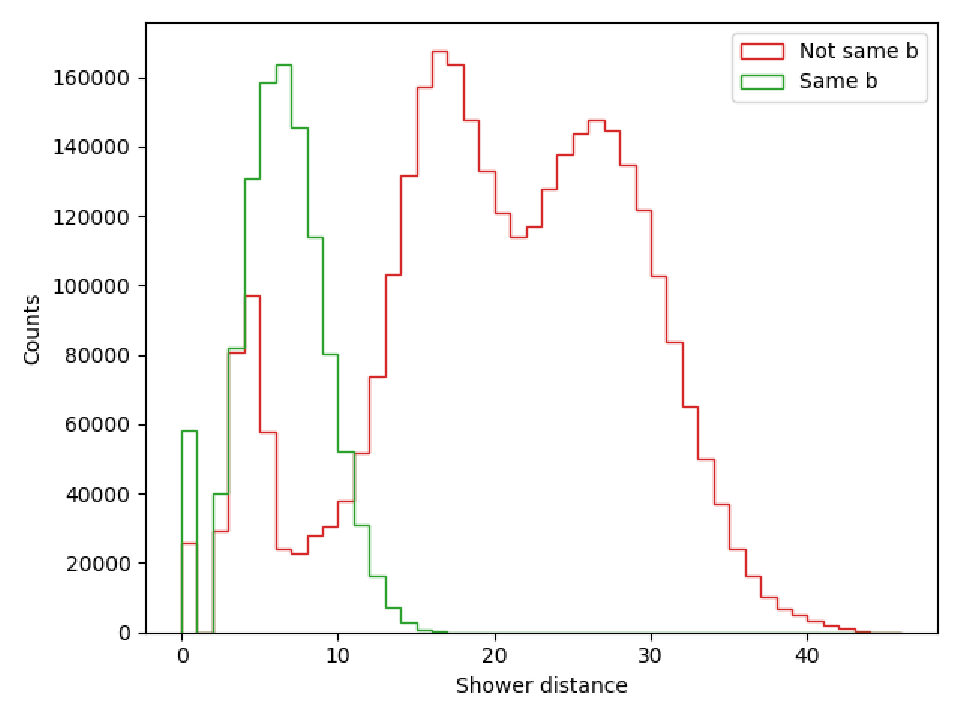
\includegraphics[width=1\textwidth]{graphics/shower_distance_example}
%    \end{minipage}\hfill
%    \begin{minipage}[c]{0.45\textwidth}
%    \caption{
%        Comparison of shower distance (see sec~\ref{sec:distance_in_eigenspace})
%        for pairs that are in the same \bthing{quark}
%        and those that are not.
%             }\label{fig:shower_distance_example}
%    \end{minipage}
%\end{figure}    
%
%The distances in physical space will be input values for affinities,
%which will be clustered subject to the aims of RatioCut, or NCut.
%As a reminder, RatioCut aims to minimise
%        \begin{equation} \text{RatioCut}(A_1 \dots A_k) = \frac{1}{2} \sum_{i=1}^k \frac{\text{cut}(A_i, \bar{A_i})}{|A_i|}\end{equation}.
%And NCut aims to minimise 
%        \begin{equation} \text{NCut}(A_1 \dots A_k) = \frac{1}{2} \sum_{i=1}^k \frac{\text{cut}(A_i, \bar{A_i})}{\text{Vol}(A_i)}\end{equation}.
%Where \(A_i\) is a point inside the cluster, and \(\bar{A}_i\) is a point outside the cluster.
%
%As the distance grows the affinity shrinks, so to have these minimise on the right groupings
%the distances between clusters should be large compared to the distances inside them.
%
%
%Three measures of this have been tried. See figure~\ref{fig:physspace_distance_comparison}.
%The first would be the ROC-AUC (Receiver Operating Characteristic - Area Under Curve),
%for the distance measure between two particles and the particles being descendent from the same
%\bthing{quark}.
%This can be thought of as a measure of how good that distance measure is at separating 
%quarks from the same \bthing{quark} from other quark pairs.
%
%The second would be the Spearman's rank of the measured distance against the Shower distance.
%Shower distance is defined by taking the simulated shower as a graph, where nodes are particles
%and vertices are interactions, and finding the least number of vertices that must be transvered 
%in order to get between the particles in the pair.
%
%\begin{figure}[htp]
%    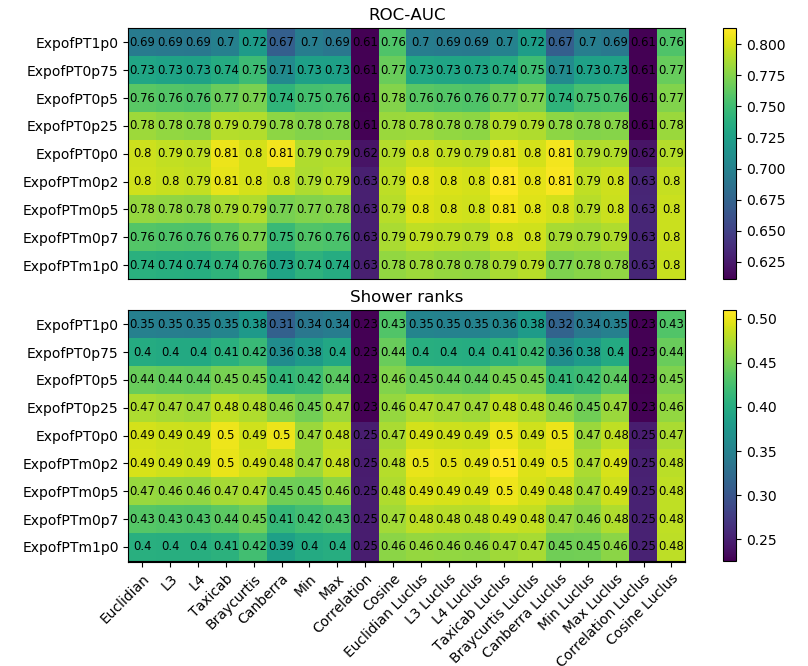
\includegraphics[width=.9\textwidth]{graphics/physspace_distance_comparison}
%    \caption{
%            Along the y axis there are jets with varying \(p_T\) exponents, going
%            from kt jets at the top, Cambridge Aachen in the middle row and anti-kt
%            on the last row.
%            On the x axis are various distance measures.
%            It seems that a Luclus PT factor is preferable.
%            The distance measures Min, Max, Correlation and Cosine
%            do not perform well, with the exception of
%            Cosine-Luclus, which works will for anti-kt jets.
%            Taxicab performs best overall, but there is not
%            a great distinction.
%             }\label{fig:physspace_distance_comparison}
%\end{figure}    
%These two are in relative agreement about which distance measures work best.
%The third is the normed distances; in each event the difference between
%the mean of distances that would be cut and the mean of distances between particle of the same
%\bthing{quark} is divided by the mean distance for that event.
%The mean of this measure over all event sis then taken.
%There seems to be some issue with this measure as it does not match well with the other two.
%It seems to prefer lower overall distances.
%
%There are \(10\) distance measures that were tried in Physical space.
%\begin{itemize}
%    \item Euclidean; \(d = \sqrt{\sum_i \delta x_i^2}\)
%    \item L3; \(d = {(\sum_i \delta x_i^3)}^{1/3}\)
%    \item L4; \(d = {(\sum_i \delta x_i^4)}^{1/4}\)
%    \item Taxicab; \(d = \sum_i |\delta x_i|\)
%    \item Braycutis; \(d = \sum_i |x_{1,i} - x_{2,i}|/\sum_i |x_{1,i} + x_{2,i}|\)
%    \item Canberra; \(d = \sum_i |x_{1,i} - x_{2,i}|/\sum_i |x_{1,i}| + |x_{2,i}|\)
%    \item Min; \(d = \text{min}_i |\delta x_i|\)
%    \item Max; \(d = \text{max}_i |\delta x_i|\)
%\item Correlation; \(d = 1 - \frac{\sum_i (x_{1,i} - \bar{x}_{1,i})(x_{2,i} - \bar{x}_{2,i})}
%                                  {\sqrt{\sum_i (x_{1,i} - \bar{x}_{1,i})^2}\sqrt{\sum_i (x_{2,i} - \bar{x}_{2,i})^2}}\)
%\item Cosine; \(d = 1 - \frac{\sum_i x_{1,i}x_{2,i}}
%                                  {\sqrt{\sum_i x_{1,i}^2}\sqrt{\sum_i x_{2,i}^2}}\)
%\end{itemize}
%
%
%A comparison of the two scoring criteria over two thousand events can be seen in figure~\ref{fig:eigenspace_distance_comparison}.
%
%\subsubsection{Distances in Eigenspace}\label{sec:distance_in_eigenspace}
%In order to test the best way to measure distance in Eigenspace a similar test to the one performed in physical space is done.
%The distance between two particles in eigenspace accordint to various metrics is co pared to both the ROC-AUC
%and the shower distance.
%%For a visualisation of these comparisons in the first event see figure~\ref{fig:eigenspace_distance_example}.
%%\begin{figure}[htp]
%%    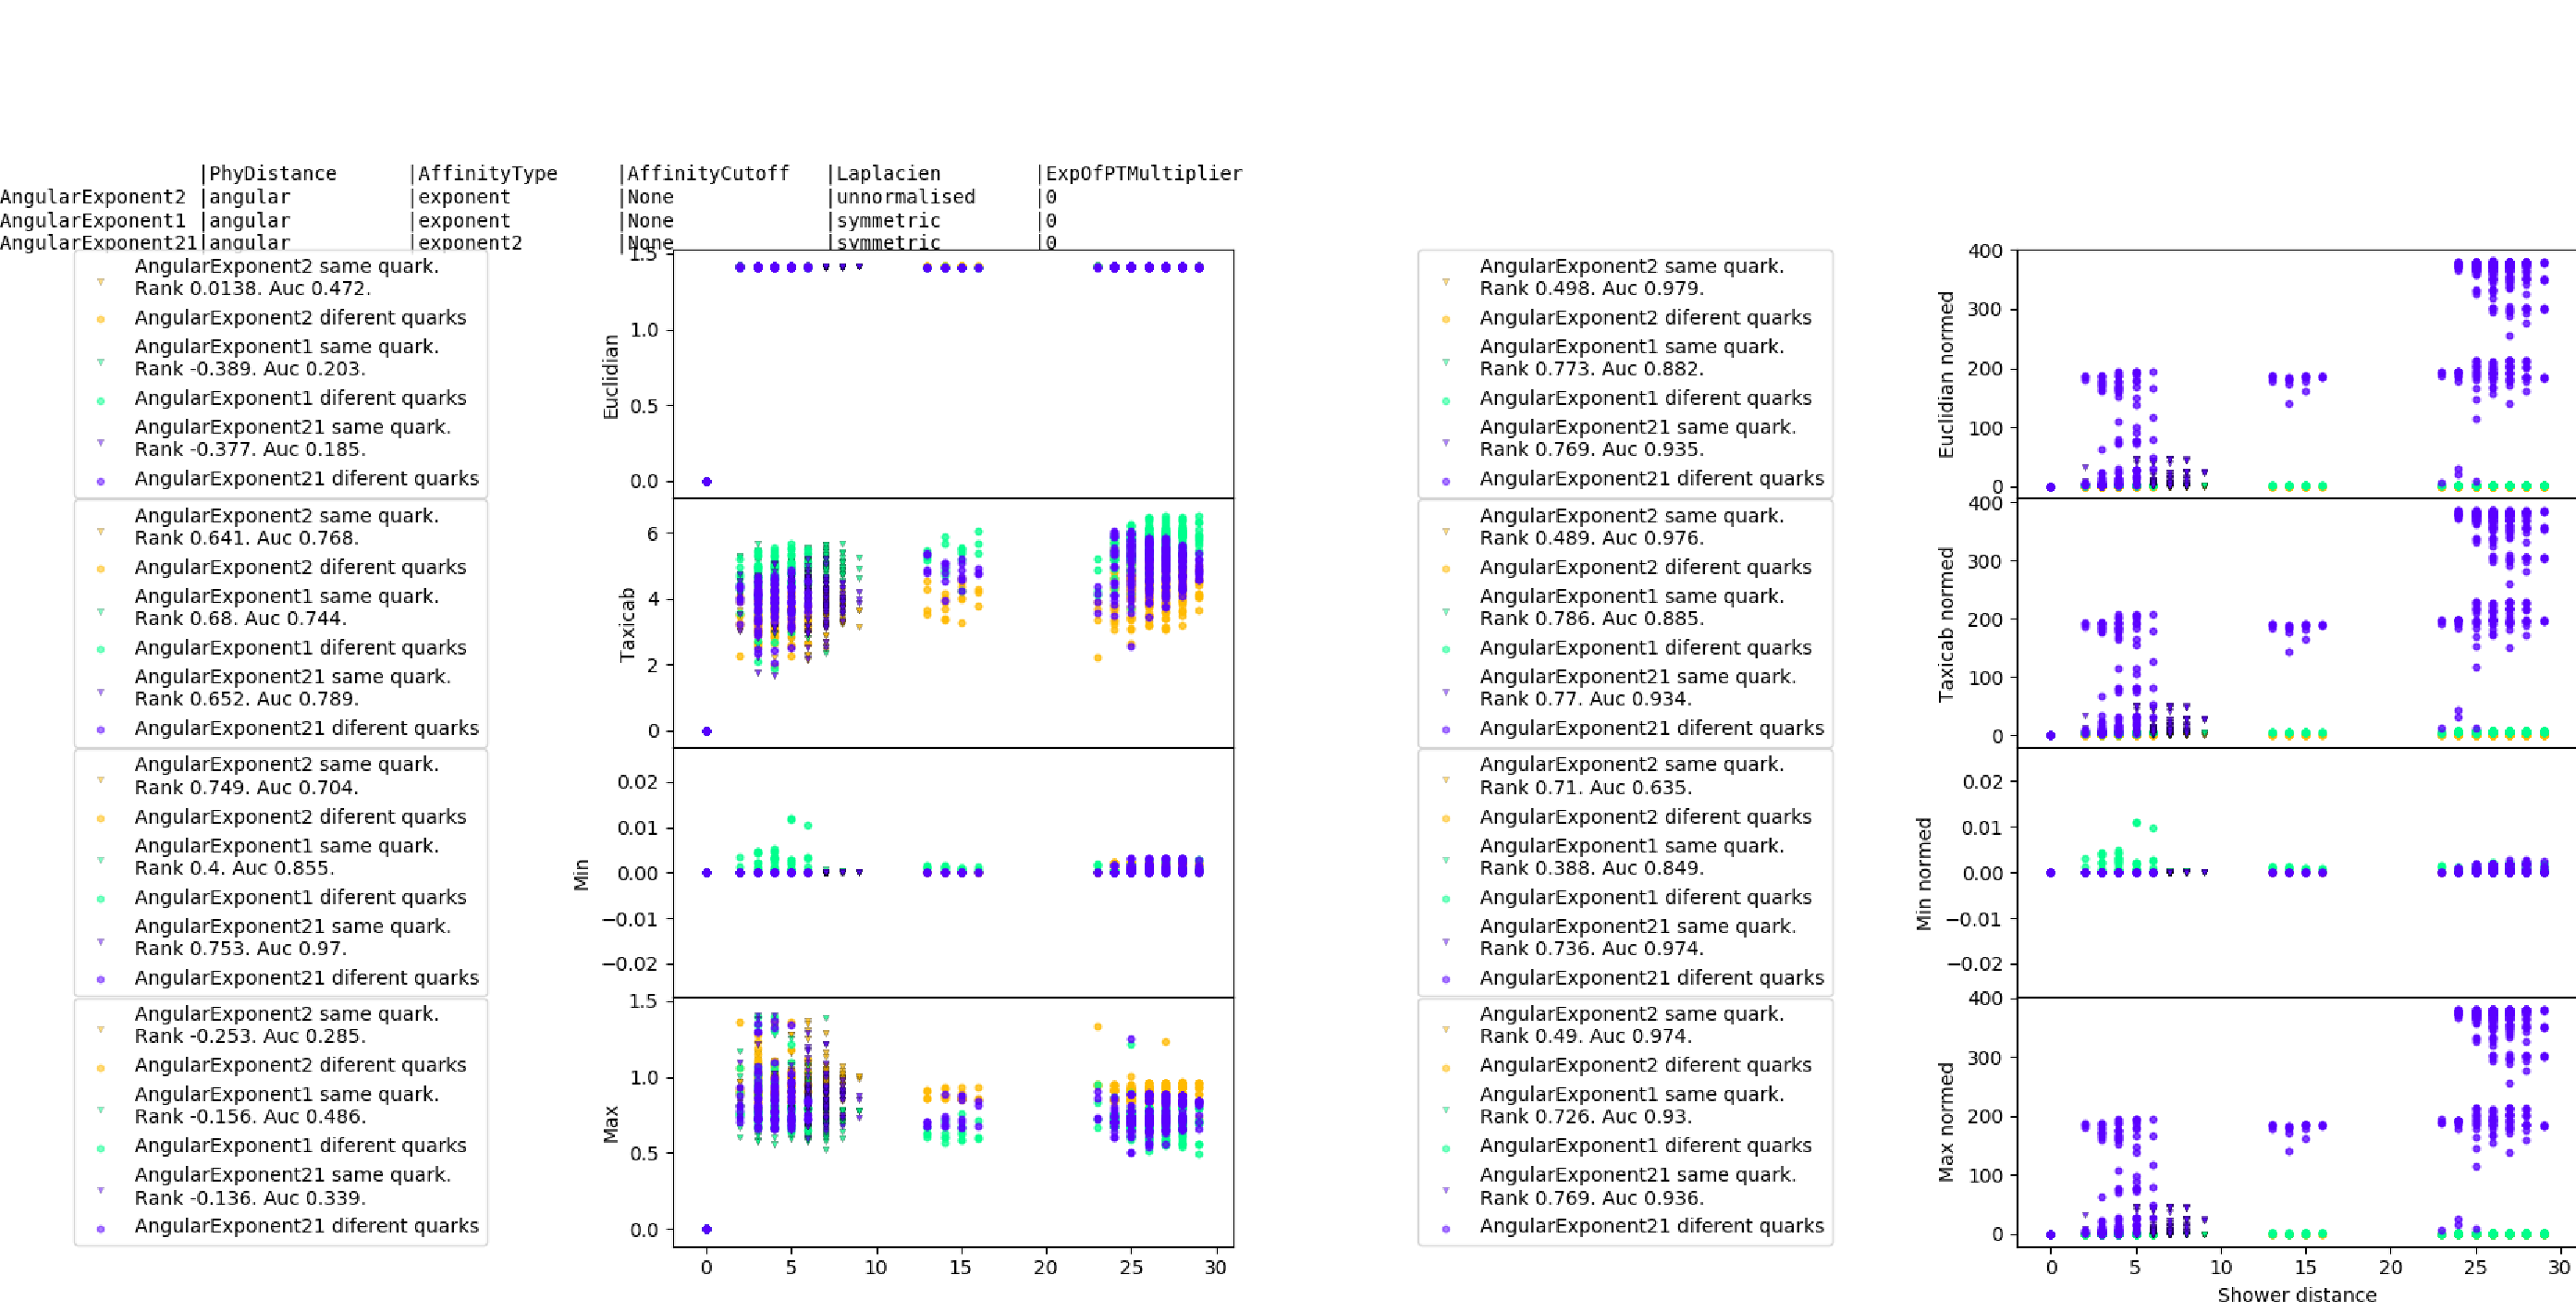
\includegraphics[width=1.\textwidth]{graphics/eigenspace_distance_example}
%%    \caption{
%%        Each plot is a comparison of shower distance (see sec~\ref{sec:distance_in_eigenspace})
%%        against a distance measure applied in the Eigenspace created at the first stage of
%%        jet formation.
%%        Each point is on a plot represents the relationship between a pair of particles
%%        that are used to form jets in the first event.
%%             }\label{fig:eigenspace_distance_example}
%%\end{figure}    
%
%There are \(10\) distance measures that were tried in Eigenspace.
%\begin{itemize}
%    \item Euclidean; \(d = \sqrt{\sum_i \delta x_i^2}\)
%    \item L3; \(d = {(\sum_i \delta x_i^3)}^{1/3}\)
%    \item L4; \(d = {(\sum_i \delta x_i^4)}^{1/4}\)
%    \item Taxicab; \(d = \sum_i |\delta x_i|\)
%    \item Braycutis; \(d = \sum_i |x_{1,i} - x_{2,i}|/\sum_i |x_{1,i} + x_{2,i}|\)
%    \item Canberra; \(d = \sum_i |x_{1,i} - x_{2,i}|/\sum_i |x_{1,i}| + |x_{2,i}|\)
%    \item Min; \(d = \text{min}_i |\delta x_i|\)
%    \item Max; \(d = \text{max}_i |\delta x_i|\)
%\item Correlation; \(d = 1 - \frac{\sum_i (x_{1,i} - \bar{x}_{1,i})(x_{2,i} - \bar{x}_{2,i})}
%                                  {\sqrt{\sum_i (x_{1,i} - \bar{x}_{1,i})^2}\sqrt{\sum_i (x_{2,i} - \bar{x}_{2,i})^2}}\)
%\item Cosine; \(d = 1 - \frac{\sum_i x_{1,i}x_{2,i}}
%                                  {\sqrt{\sum_i x_{1,i}^2}\sqrt{\sum_i x_{2,i}^2}}\)
%\end{itemize}
%And each of these was reattempted after the eigenspace had been ``normed" by 
%dividing each eigenvector by it's eigenvalue.
%This creates \(20\) possible ways to measure distance in Eigenspace.
%
%
%A comparison of the two scoring criteria over two thousand events can be seen in figure~\ref{fig:eigenspace_distance_comparison}.
%\begin{figure}[htp]
%    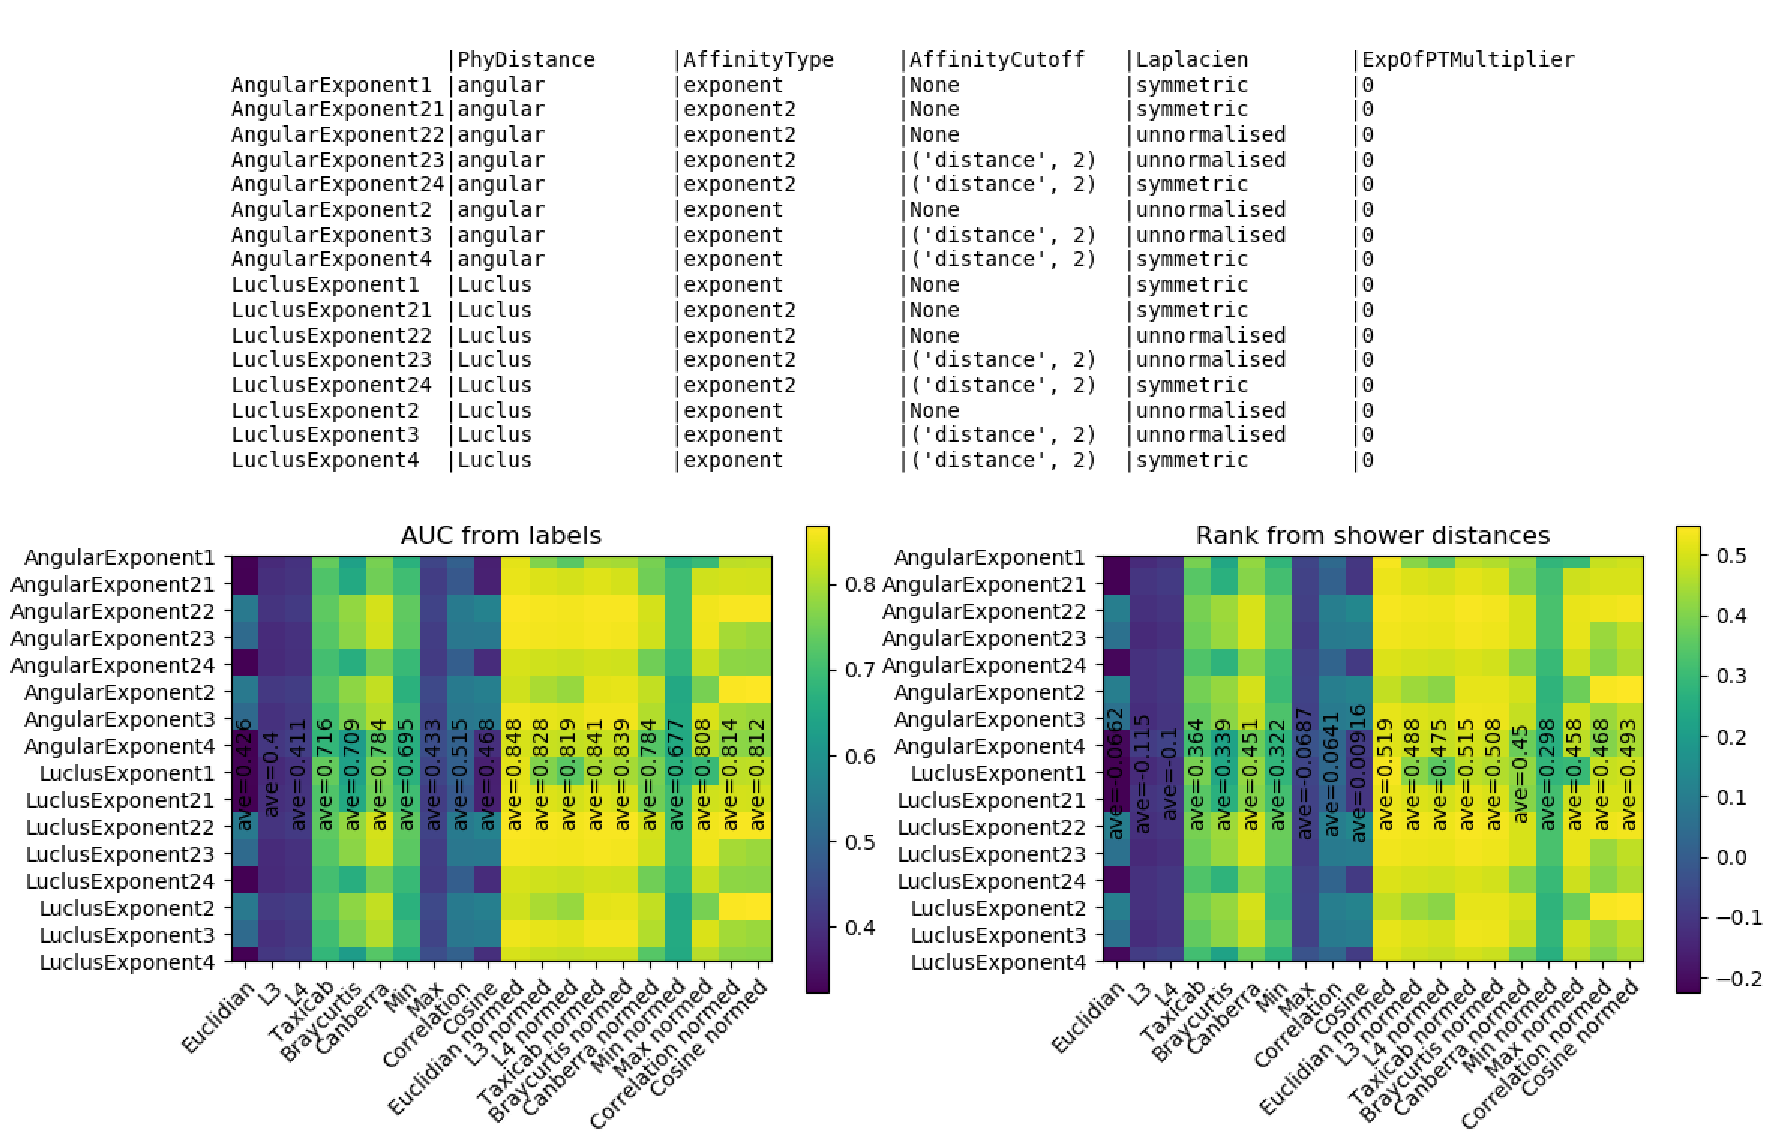
\includegraphics[width=1.\textwidth]{graphics/eigenspace_distance_comparison}
%    \caption{
%        The plots are heatmaps with various jet clustering approaches on
%        the y axis and different ways to measure the distance in eigenspace on the
%        x axis (see sec~\ref{sec:distance_in_eigenspace}).
%        The left and plot is the ROC-AUC (measure closet to our aim)
%        the right hand plot is the shower distance (measure easiest to interpret physically).
%        Both plots are in strong agreement.
%        It is clearly important to norm the eigenstate, and either Euclidean or Taxicab distance
%        are equally acceptable with Euclidean results being marginally stronger.
%             }\label{fig:eigenspace_distance_comparison}
%\end{figure}    
